\chapter{实验结果与分析}
本章将对实验进行检验并对比分析:将统计各个类的AP值并做出PR曲线;预测效果展示,并展现其中效果不佳的结果;探究实验泛化性能力。
\section{实验平台}{
	基本环境:
	\begin{enumerate}
		\item 操作系统: CentOS Linux release 7.1
		\item 显卡: GTX1080
		\item CUDA版本: 8.0
		\item 实验框架: Darknet
		\item 数据集: KITTI
	\end{enumerate}

	YOLO训练参数:
	\begin{enumerate}
		\item batch size: 64
		\item width: 416
		\item height: 416
		\item channels: 3
		\item momentum: 0.9
		\item decay: 0.0005
		\item learing rate: 0.001
		\item max batches: 50000
	\end{enumerate}

	tiny-YOLO训练参数:
	\begin{enumerate}
		\item batch size: 64
		\item width: 416
		\item height: 416
		\item channels: 3
		\item momentum: 0.9
		\item decay: 0.0005
		\item learing rate: 0.001
		\item max batches: 50000
	\end{enumerate}

	如图\ref{trainYOLO}、\ref{trainTiny-YOLO},展现了两个模型的训练过程。

	\begin{figure}[htbp]
	\centering
	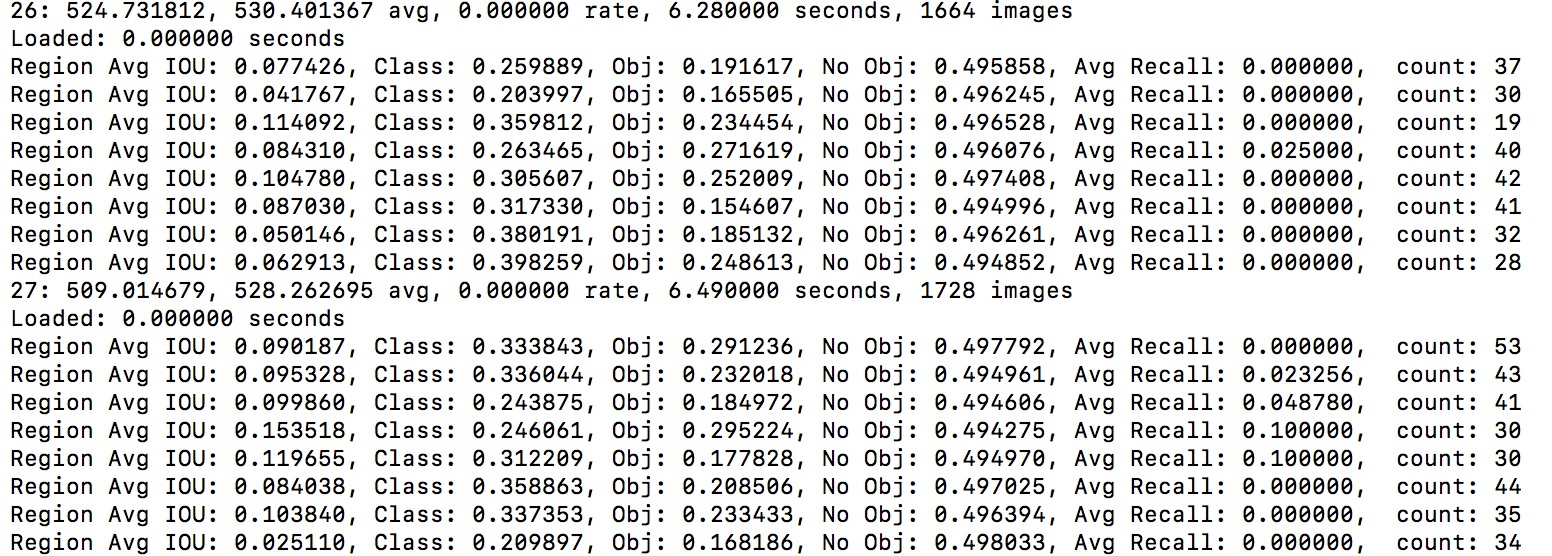
\includegraphics[width=5in]{images/trainYOLO.png}
	\caption{YOLO训练过程}
	\label{trainYOLO}
	\end{figure}
	\begin{figure}[htbp]
	\centering
	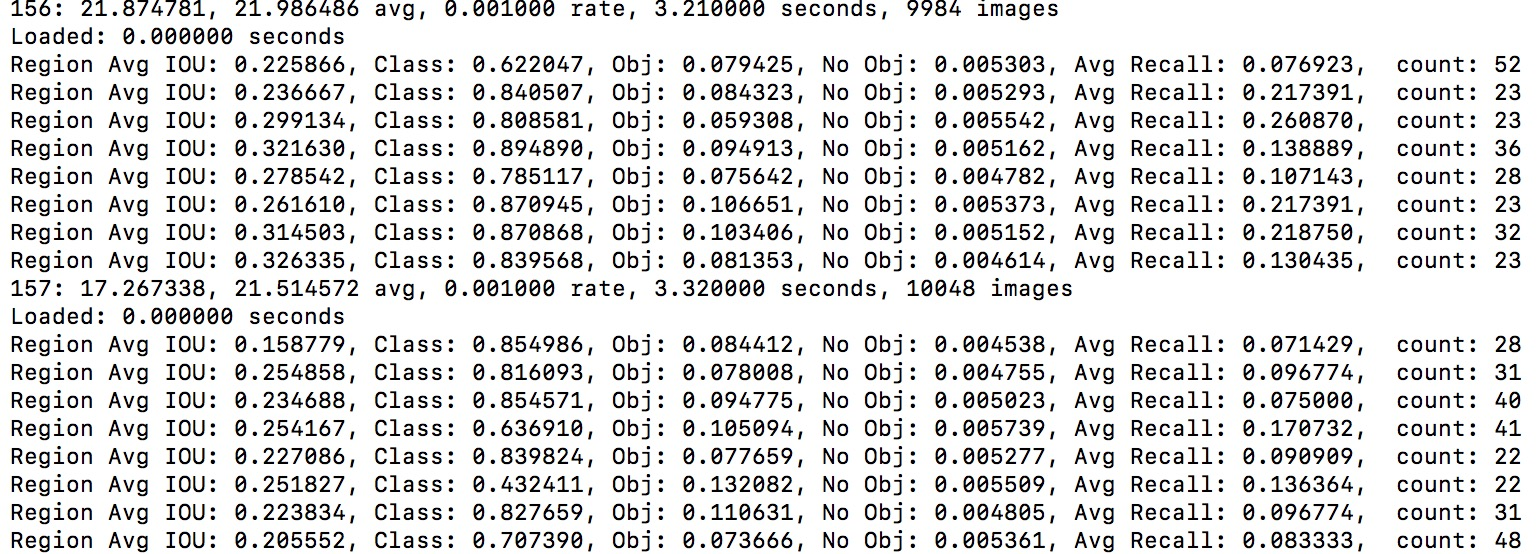
\includegraphics[width=5in]{images/trainTiny-YOLO.png}
	\caption{tiny-YOLO训练过程}
	\label{trainTiny-YOLO}
	\end{figure}
}

\section{结果对比}{
	\subsection{AP比较}
	\begin{table}  
	\caption{各模型各类AP和FPS结果对比}  
	\begin{tabular}{l|p{2cm}p{2cm}p{2cm}p{2cm}}  
	\hline  
	             & Pedestrian & Car      & Cyclist  & FPS \\  
	\hline  
	Faster R-CNN & 65.91 \%   & 79.11 \% & 62.81 \% & 5   \\  
	YOLO         & 51.44 \%   & 68.05 \% & 50.97 \% & 45  \\
	tiny-YOLO    & 26.67 \%   & 50.75 \% & 25.04 \% & 120 \\
	\hline
	\end{tabular}
	\label{AP}
	\end{table} 
	我们首先对比本项目各个模型对于各个类的AP值以及FPS比较,如表\ref{AP}。其中Faster R-CNN的数据参考自\cite{}。

	通过图表,我们可以发现虽然tiny-YOLO有120fps,而yolo只有45fps,比YOLO的速度快上2-3倍,但是性能远不如YOLO。从速度上来看,YOLO能达到每秒45帧的速度,已经基本可以满足实时行人检测的需求,tiny-YOLO甚至然能够达到每秒120帧的速度,两个模型均能满足实时行人检测的要求。从性能上来看,不管是哪个类的AP值,YOLO都全面领先于tiny-YOLO,尤其是在行人和自行车的检测上,而YOLO不仅在行人和自行车上能分别达51.44AP和50.97AP,在车辆检测上更是能达到68.05AP,效果较好。而反观tiny-YOLO,它在车辆检测上只有50.75AP,而在行人检测和自行车检测上更是仅有26.67AP和25.04AP

	从整体上看,模型对车辆的检测明显高于对行人和自行车的检测,这是由于KITTI数据集中车辆数据较多造成的。而模型的整体表现也部分受限于训练数据过少。

	对比Faster R-CNN,Faster R-CNN仅有5fps,无法满足实时行人检测的要求,不管是YOLO还是tiny-YOLO,在速度上都明显比Faster R-CNN要快上很多。并且Faster R-CNN在行人、车辆、自行车上的检测分别有65.91AP、79.11AP、62.81AP,YOLO在这三项上的损失并没有想象上的那么大。可见YOLO仅牺牲了部分的精度确在检测速度上提高了很多。

	总的来说,YOLO在AP上的表现达到预期效果,而tiny-YOLO虽然速度很快,但是效率上损失过多。

	\subsection{PR曲线比较}
	\begin{figure}[htbp]
	\centering
	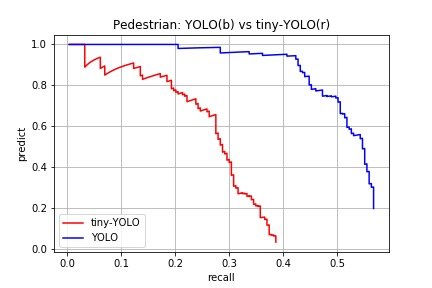
\includegraphics[width=5in]{images/pedestrianPR.png}
	\caption{行人检测比较}
	\label{pedestrianPR}
	\end{figure}
	\begin{figure}[htbp]
	\centering
	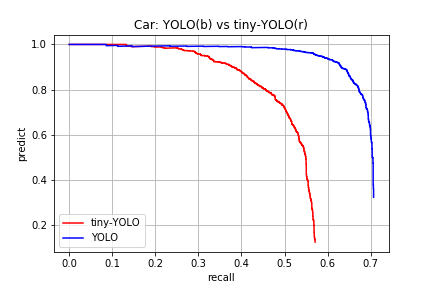
\includegraphics[width=5in]{images/carPR.png}
	\caption{车辆检测比较}
	\label{carPR}
	\end{figure}
	\begin{figure}[htbp]
	\centering
	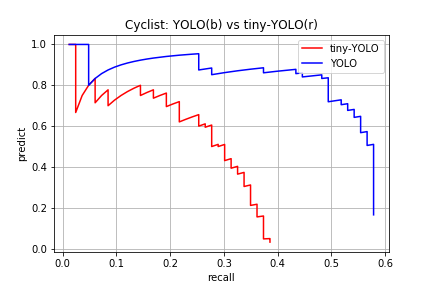
\includegraphics[width=5in]{images/cyclistPR.png}
	\caption{自行车检测比较}
	\label{cyclistPR}
	\end{figure}
	我们分别对各个模型各个类做出PR曲线并进行比较,结果如图\ref{pedestrianPR}、\ref{carPR}、\ref{cyclistPR}。

	从图\ref{pedestrianPR}中可以看出,对于行人的检测上,YOLO模型明显好于tiny-YOLO的模型,在召回率0.4的时候,tiny-YOLO的准确率已经接近0,而YOLO的准确率还是接近1。

	从图\ref{carPR}中可以看出,对于车辆的检测,两个模型都有很好的表现,PR曲线都很飘。tiny-YOLO大概在召回率大于0.45后准确率开始快速下降,而YOLO则在召回率大于0.6后准确率快速下降。

	从图\ref{cyclistPR}中可以看出,对于自行车的检测,YOLO模型也明显好于tiny-YOLO模型。tiny-YOLO下降速度比较稳定,而YOLO在召回率大于0.5后准确率开始快速下降。
}

\section{预测效果}{
	\subsection{效果展示}
	\begin{figure}[htbp]
	\centering
	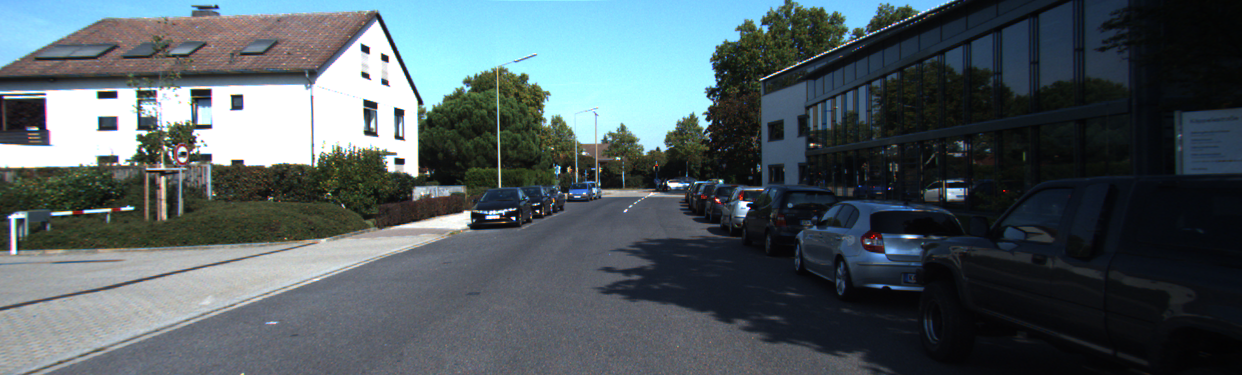
\includegraphics[width=5in]{images/007435.png}
	\caption{输入图像}
	\label{007435}
	\end{figure}
	我们选择了一张情形较为复杂的图作为输入,如图\ref{007435}。

	\begin{figure}[htbp]
	\centering
	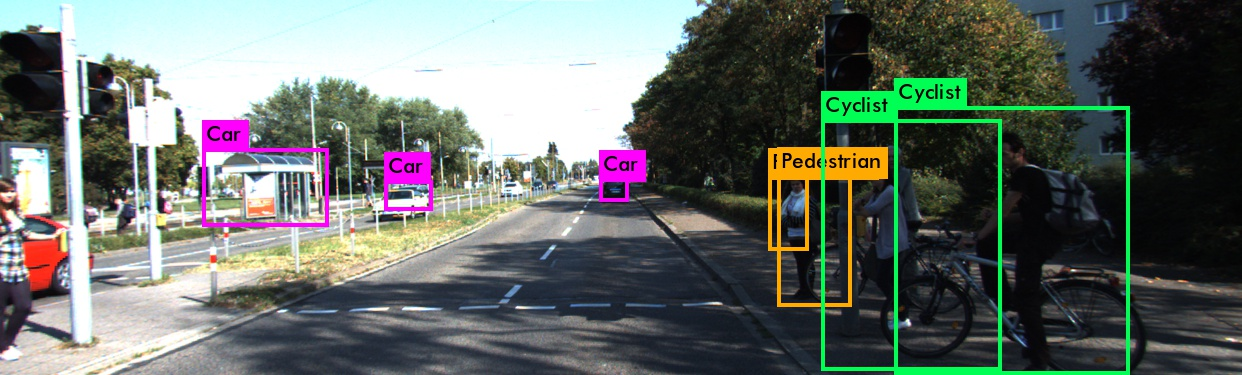
\includegraphics[width=5in]{images/predictYOLO.jpg}
	\caption{YOLO预测结果}
	\label{predictYOLO}
	\end{figure}
	\begin{figure}[htbp]
	\centering
	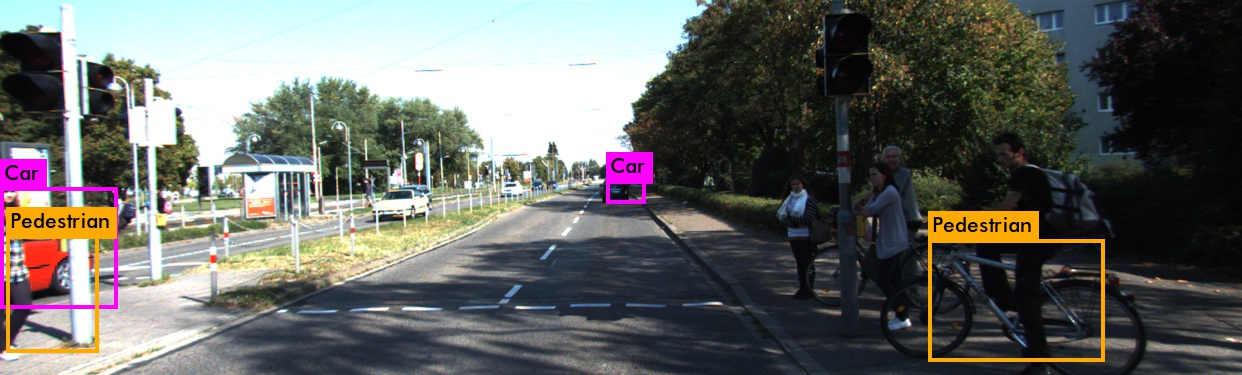
\includegraphics[width=5in]{images/predictTiny-YOLO.jpg}
	\caption{tiny-YOLO预测结果}
	\label{predictTiny-YOLO}
	\end{figure}

	测试结果如图\ref{predictYOLO}、\ref{predictTiny-YOLO}所示。YOLO的测试结果中,预测出来的结果基本正确,而且预测框很好的覆盖了物体,不过其中出现了两个错误,一个是重复预测了一个行人,一个是将公交车站预测成为了车辆;另外一些不完整的车辆和行人没有预测出来。而tiny-YOLO的情况就较为差了,很大一部分容易预测出来的物体并没有成功检测到,将自行车预测成行人,预测框与物体的真值框差别较大。

	从上述分析中我们可以看出YOLO基本能满足行人检测的要求,而tiny-YOLO的检测性能过低就不太适合了。另外使用YOLO网络对不完整的物体检测性能不佳,有重复检测情况,对过于细小的物体检测不佳(大部分模型对过于细粒度物体的检测都不太支持)。

	\subsection{错误结果分析}
	我们分别检测了YOLO模型在细小物体靠的近时候的表现以及不完整物体的表现。

	\begin{figure}[htbp]
	\centering
	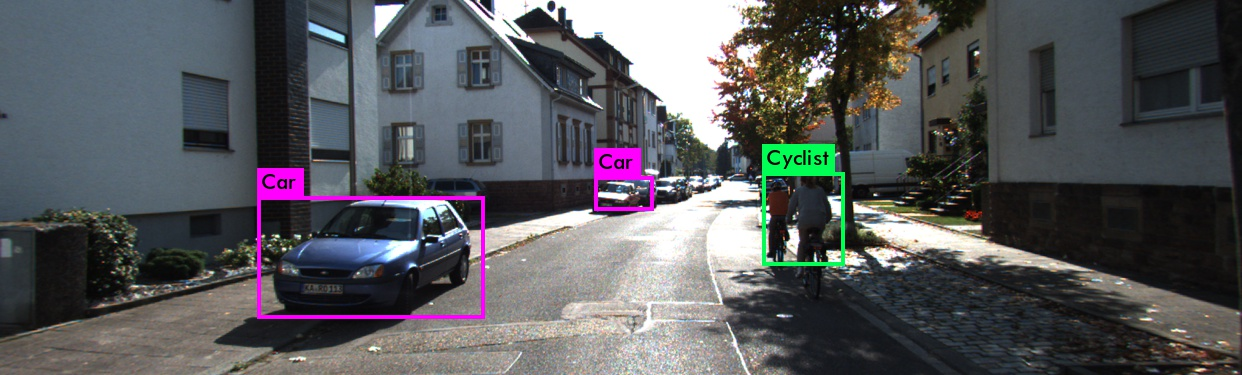
\includegraphics[width=5in]{images/error1.jpg}
	\caption{细小集群的测试}
	\label{error1}
	\end{figure}
	如图\ref{error1},YOLO队友两个靠的很近骑自行车的人检测成了一个骑自行车的人,这主要是由于YOLO将物体检测分为了S*S的方格,而多个细粒度的物体如果在一个方格内的话,YOLO会很容易将多个物体检测成一个物体。所以YOLO对细粒度的集群检测性能不佳。

	\begin{figure}[htbp]
	\centering
	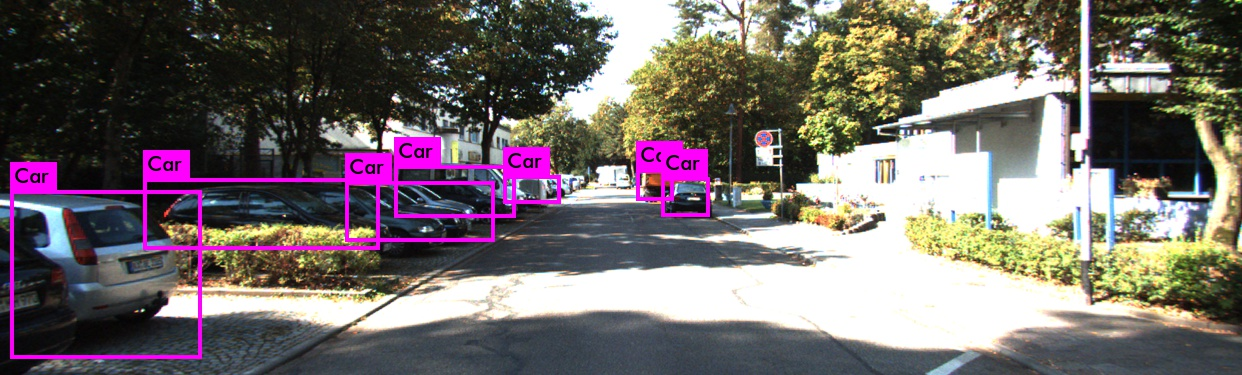
\includegraphics[width=5in]{images/error2.jpg}
	\caption{不完整物体的测试}
	\label{error2}
	\end{figure}
	如图\ref{error2},YOLO对不完整物体的检测没有想象中的糟糕,对于大部分不完整的物体还是能够准确检测出来的,除开该物体残缺部分过多。另外由于YOLO对细小集群表现不佳,物体间的覆盖也会导致检测的性能损失。

	\begin{figure}[htbp]
	\centering
	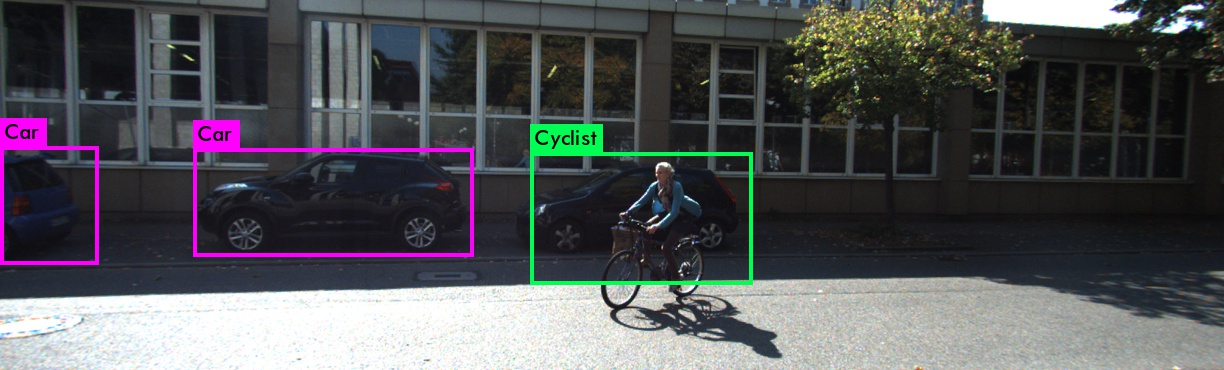
\includegraphics[width=5in]{images/error3.jpg}
	\caption{不同物体覆盖的测试}
	\label{error3}
	\end{figure}
	如图\ref{error3},YOLO对不同物体的覆盖检测性能不佳。该问题与YOLO对细小集群检测不佳的问题类似,这是由于YOLO把检测问题分为S*S的方格,而每个方格只预测其中一个具体的类,如果不同物体产生覆盖现象,往往不能同时预测成功出这些不同的物体来。
}

\section{泛化性}{
	本项目讨论实时行人检测的可行性,针对日常生活驾驶、极端天气、夜晚等各种情形进行实验。

	\begin{figure}[htbp]
	\centering
	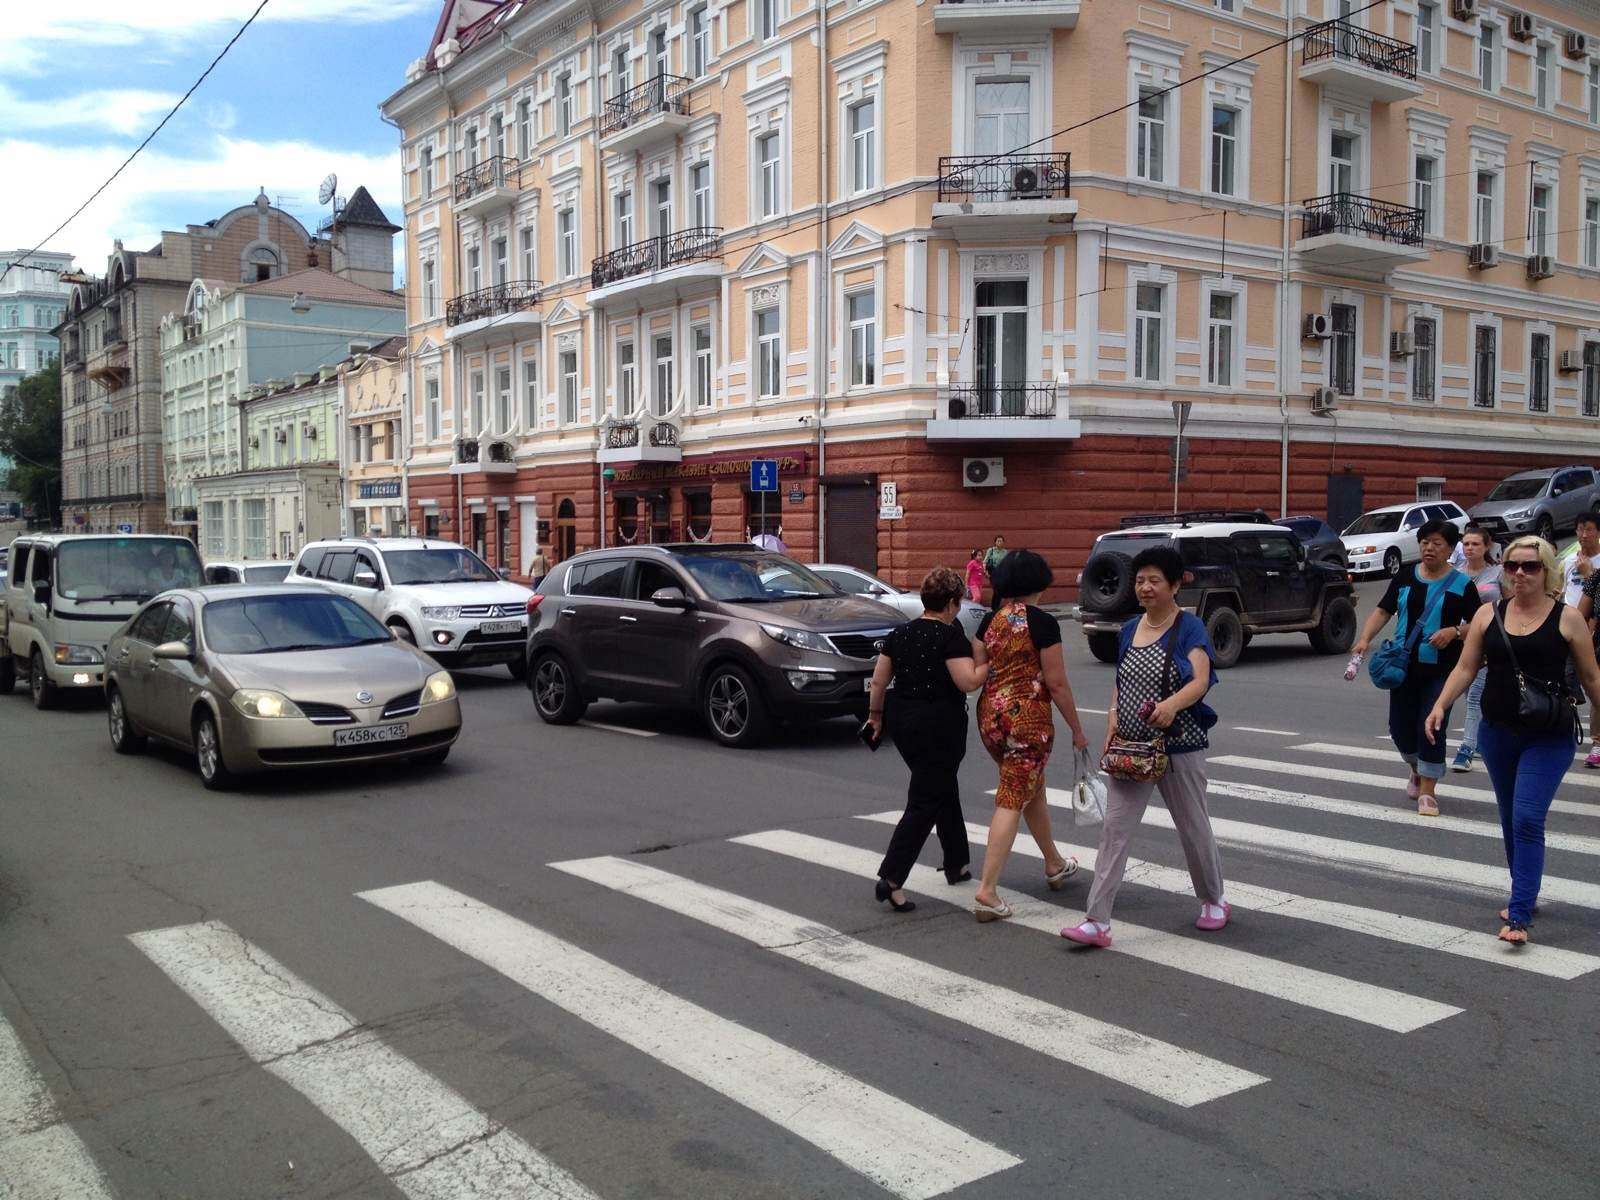
\includegraphics[width=5in]{images/daily.jpg}
	\caption{日常生活驾驶}
	\label{daily}
	\end{figure}
	\begin{figure}[htbp]
	\centering
	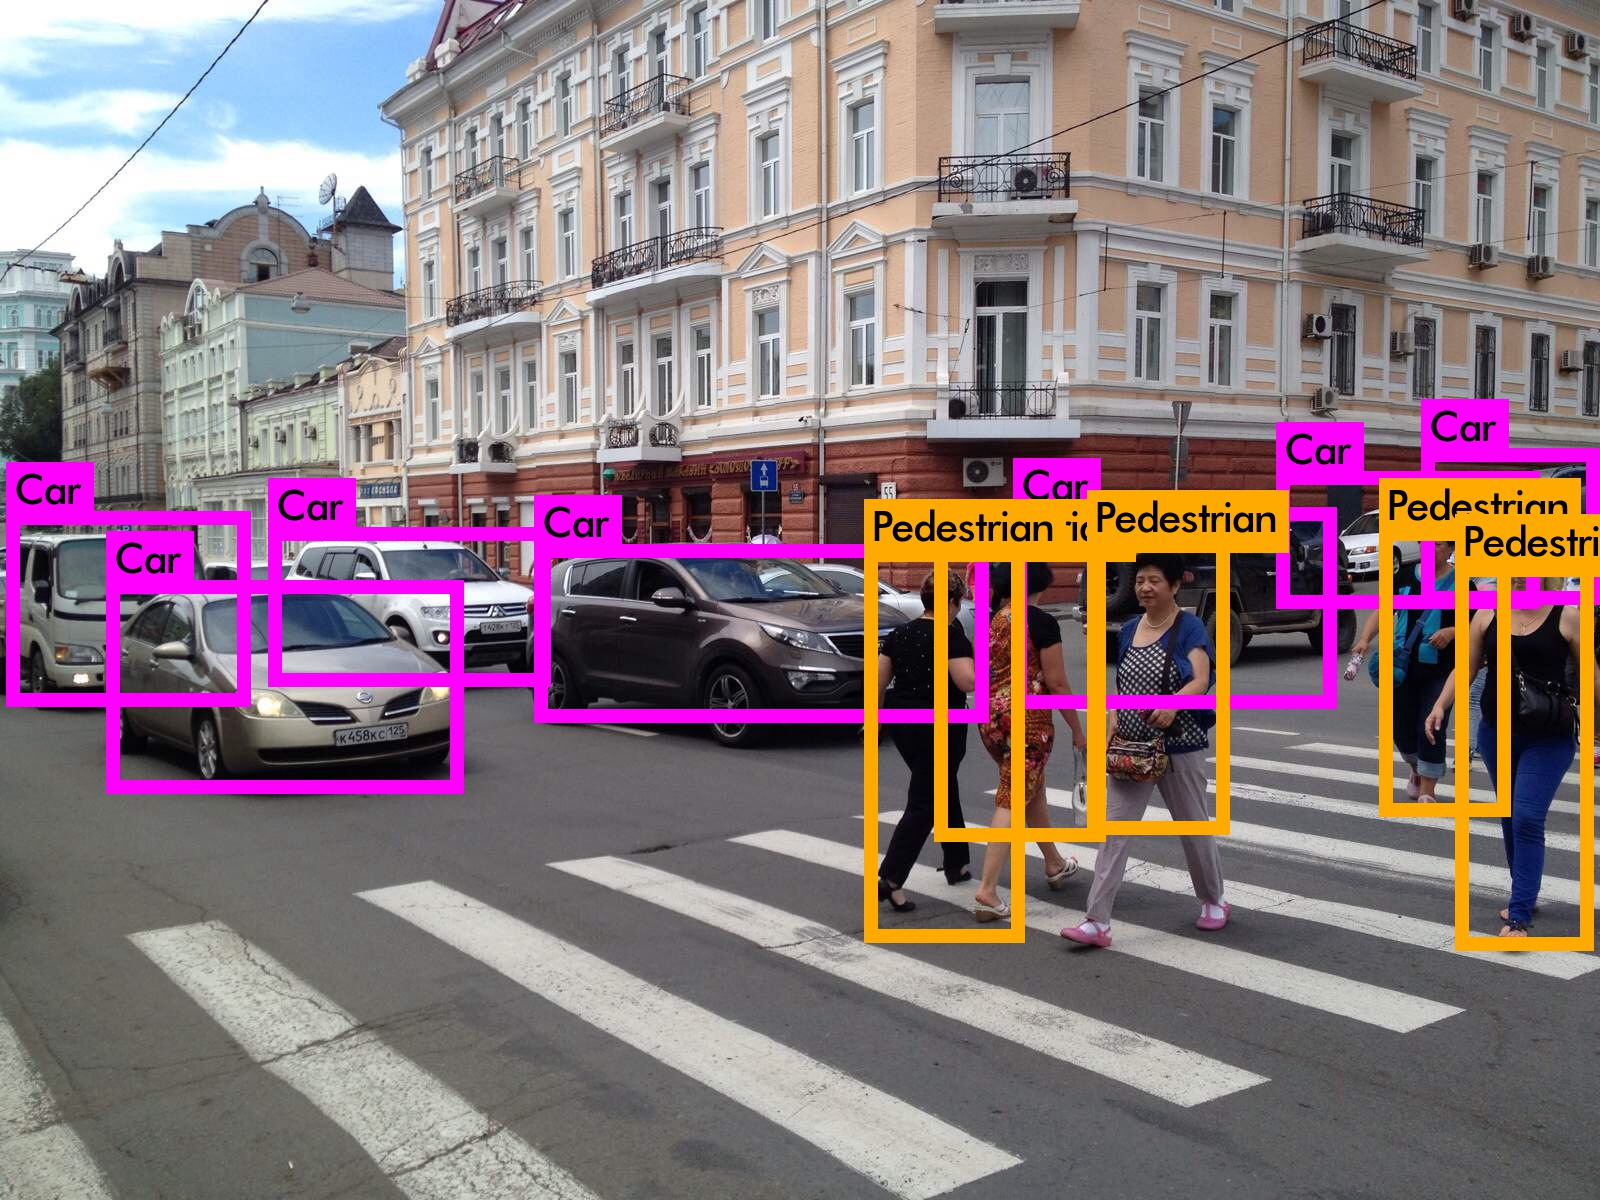
\includegraphics[width=5in]{images/predictDaily.jpg}
	\caption{日常生活驾驶预测结果}
	\label{predictDaily}
	\end{figure}
	我们针对日常生活驾驶过程中的情况做了测试,测试输入如图\ref{daily},预测结果如图\ref{predictDaily}。模型对正常驾驶情况下的预测性能很好,基本能够满足实时行人检测的要求。

	\begin{figure}[htbp]
	\centering
	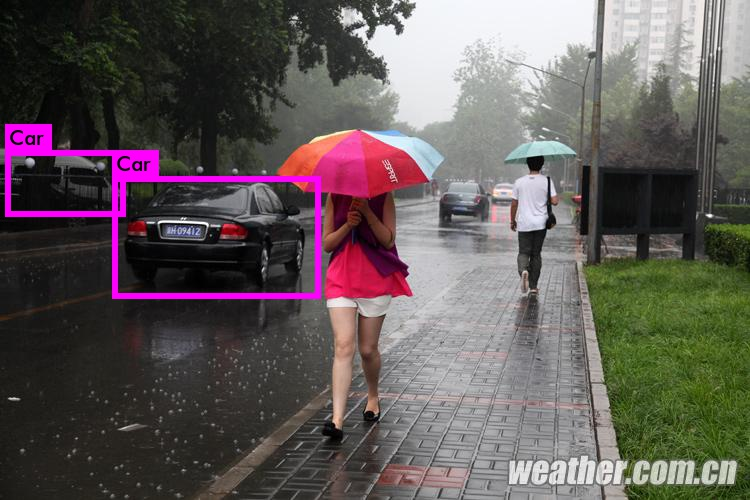
\includegraphics[width=5in]{images/rain.jpg}
	\caption{雨中行人检测}
	\label{rain}
	\end{figure}
	\begin{figure}[htbp]
	\centering
	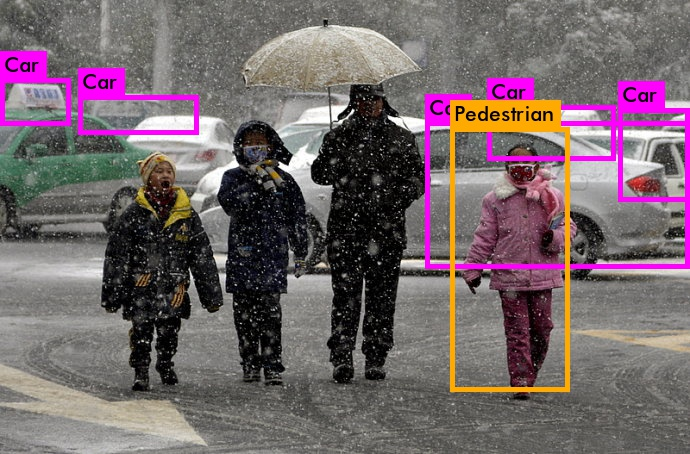
\includegraphics[width=5in]{images/snow.jpg}
	\caption{雪中行人检测}
	\label{snow}
	\end{figure}
	我们针对极端天气情况进行了泛化性测试,结果如图\ref{rain}、\ref{snow}。从图中可以看出,模型对极端天气情况下表现较差,对于雪中的预测,可能是主要受到噪声(雪)的干扰,所以行人和车辆预测效果都不佳;对于雨中的预测,则可能是受到行人拿伞的影响,所以对行人检测性能不佳但是对车辆检测性能还行。

	\begin{figure}[htbp]
	\centering
	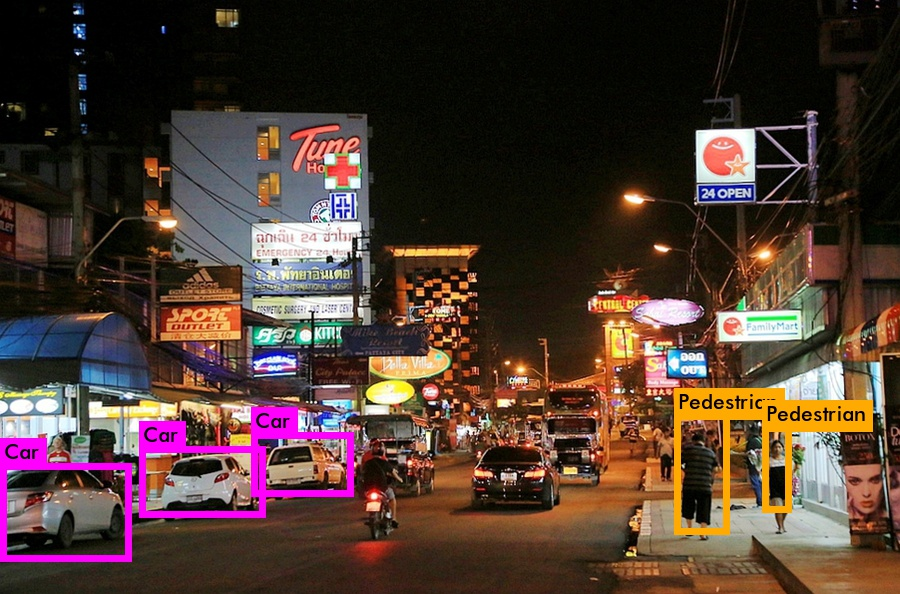
\includegraphics[width=5in]{images/night.jpg}
	\caption{夜晚行人检测}
	\label{night}
	\end{figure}
	我们针对夜晚的情况进行了泛化性测试,结果如图\ref{night}。从图中可以看出,模型对夜晚情况下行人和车辆的检查性能还行,虽然还是远不如正常情况下的行人检测,但是已经能够说明模型能在夜晚或光照不好的情况下进行行人检测。
}

\section{本章小结}{
	本章对本项目做了详细的实验和分析。我们首先介绍了我们的实验环境和训练参数等。接着,我们研究了各个模型的AP、FPS值和PR曲线,对比分析得到YOLO网络基本满足实时行人检测的要求。之后我们具体分析了预测的效果以及错误结果的分析,分析出了YOLO进行行人检测的一些弊端。最后我们对模型进行了泛化性的检验,检验结果表明虽然对于极端天气情况下模型表现不佳,但是总体而言模型的泛化性程度较高。通过实验,我们探究了模型的实时行人检测的能力和不足。
}


